\author{Bautrelle Fotso}
\graphicspath{ {./src/chapters/developer/media/} }

\section{Correction process and application of the AI: \emph{Predict\_interface}}

\subsection{Predicting using EMNIST and MNIST models}
In this section, the entire corrections cycle from the frontend through the backend and back to the frontend will be presented.
But the essential point is to know, how the prediction interface comes in action during this procedure. 

The \emph{predict\_interface} is the intermediate stage between the preprocessing and the Artificial Intelligence (AI), 
where the models obtained when training the network will be used for the prediction. 
This interface firstly contains a function to enlarge each image to 28x28 pixels 
by padding its margings with zeros. The preprocessing uses this function to resize the cropped image of the text previously selected
in frontend before predicting it. This step is very important because the size of the image is an essential factor for a model to work.
The function have been performed to reshape images to 28x28 pixels since many networks for image classification works with images of this pixels shape.

\noindent
The second main function in this network is the prediction function. In this function all built models are loaded. 
Mapps are also defined as already described in the chapter about datasets. 
The prediction will be done for each task\_type according to the type of exercises being corrected, precisely exercises with number,
text or text without number.

\begin{itemize}
    \item \textbf{Number}
\end{itemize}
When the type of the exercise is a \emph{number}, the MNIST model is used in this case to predict the given image.The image will firstly be 
resized to have the dimension 28x8x1 because the function enlarge\_image() reshaped it to a 28x28 image. But this shape as said above, is only 
compatible with the DFFNN on which the MNSIT model has been built. EMNIST-digits model can then be used to predict the new resized image. 

\begin{itemize}
    \item \textbf{Text}
\end{itemize}
When the exercise is rather a \emph{text}, the EMNIST-balanced and the EMNIST-byMerge model are used to predict the image. 
In this case, the image reshaping is also 
needed because the two models are obtained from the 2D-CNN model. Since this datasets have both letters and digits they are therefore 
adequate for the recognition of such exercises. 

\begin{itemize}
    \item \textbf{text\_without\_number}
\end{itemize}
When the exercise is a \emph{text\_without\_number}, two options of recognition possible are the EMNIST\_letters model and the tesseract 
model. More about tesseract is explained in the following subsection.
\hfill \break

\noindent  
The figure(\ref{Abb:ki_application})  illustrates the entire process of the correction of an exercise 
and how the predict\_interface intervenes during this procedure.

\begin{figure}[htb]
	\centering
	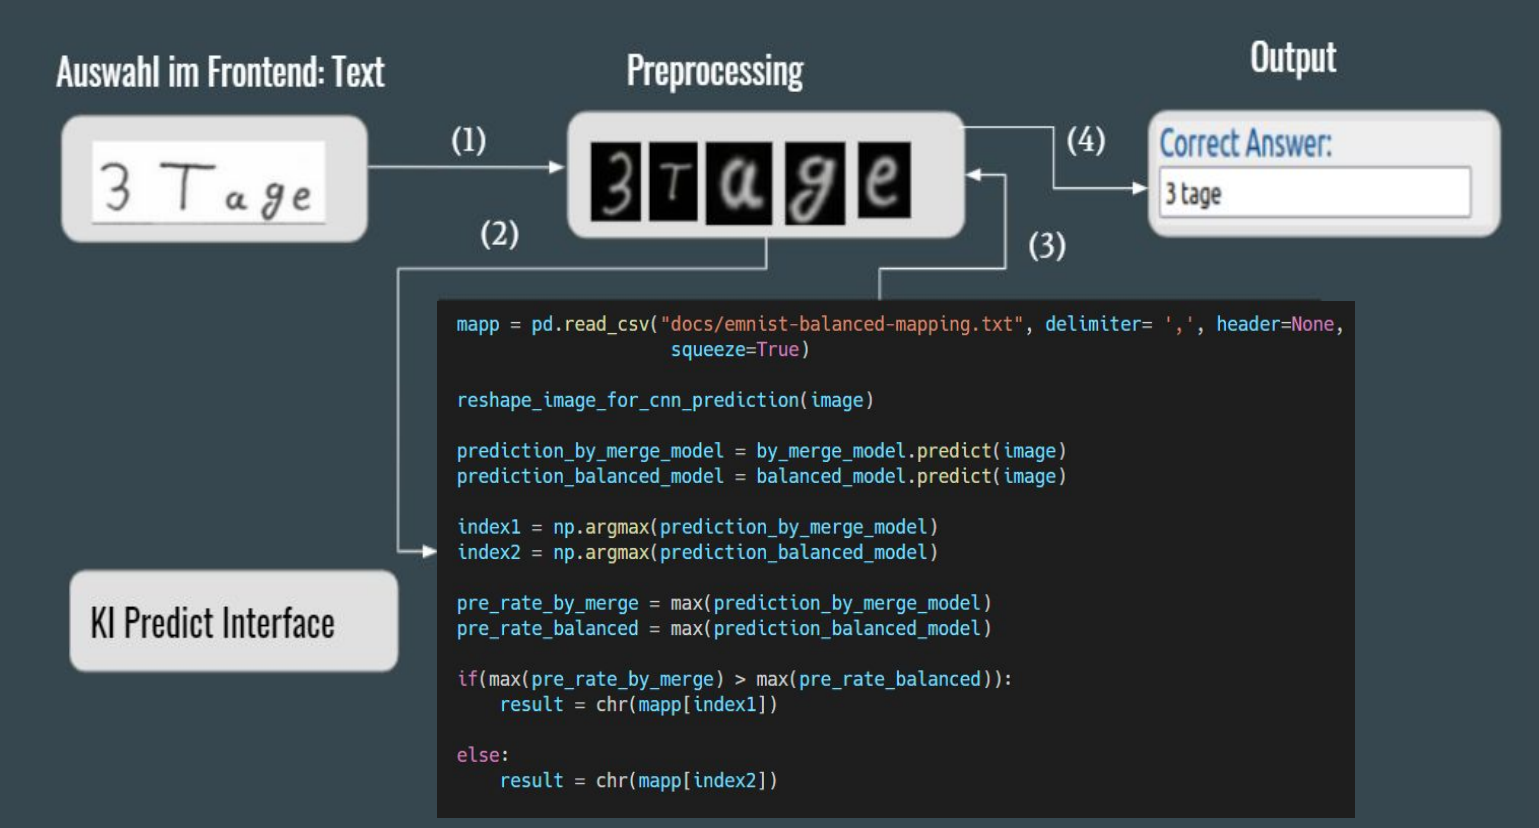
\includegraphics[width=1.0\textwidth]{prediction_text}
	\caption[Prediction interface]{Application of AI in the corrections cycle} \label{Abb:ki_application}
\end{figure}

\noindent
The example on the above picture is based on the recognition of a small text on an exam paper. 
The area of the text is first snipped on the frontend 
plattform and sent to the web-backend, especially to the preprocessing interface. 
Reaching this stage, the image will be edited for example by grayscaling it in order to get a binary image, 
which promotes a better recognition of the image. 
Each character will then be cropped and sent to the \emph{predict\_interface} function. 
Once in the prediction interface, each image character will be resized using the function 
\emph{reshape\_image\_for\_cnn\_prediction} to make it compatible with the 2D-CNN models used here. 
After rescaling, each model will predict the resized image characters. 
The result can be a 2D-array of probabilities made on the predicted character according to the 47 classes of the two datasets 
represented in the variable mapp. 
As the name already indicates, the variable \emph{mapp} describes all type of classes available in a dataset. 
An illustration of the predictions obtained for the last character which is "e" is shown in the figure(\ref{Abb:predicted_value}). 

\begin{figure}[htb]
	\centering
	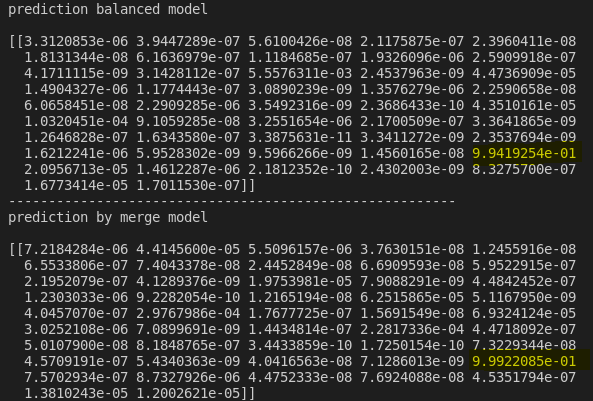
\includegraphics[width=0.8\textwidth]{predicted_value}
	\caption[Prediction output]{predictions of the character image \emph{e} on balanced and by\_merge dataset} \label{Abb:predicted_value}
\end{figure}

\noindent
The maximum of each of the above matrix will be determined by using the function \emph{numpy.amax()}. 
As seen in the figure above the 
EMNIST\_by\_merge model has a higher prediction than the EMNIST-balanced model.
The index of the highest value in the EMNIST\_by\_merge prediction corresponds to the index in the mapp
(index 101) which value is the letter "e" in ascii representation. 

\noindent 
When all images are predicted, they are sent back to the preprocesing interface which 
join them together and a whitespace is added if necessary to form a string. This string is endly
forwarded to the frontend. For this example the correct answer is "3 Tage" as expected.

\subsection{Predicting using tesseract-ocr}
To predict with tesseract, there is no need to crop each character because tesseract can work on whole words or block of text.
After the image have been cropped on the frontend, it is sent to the preprocessing interface which directly send it to the 
prediction interface in order to be recognised using tesseract.

\noindent
Using the function \emph{image\_to\_string} from the \emph{pillow} python module, the image is first converted to an array 
in the predition interface. 
This conversion is needed because the option \emph{image\_to\_string} of \emph{pytesseract} takes an array as input. 
With some specific options the cropped image will be predicted and the output will be sent back to the preprocessing interface. 
These options are: 
\begin{itemize}
    \item \emph{oem} for \textbf{ocr engine mode}, an option for different networks availble for tesseract
    \item \emph{psm} for \textbf{page segmentation mode}, an option to tell tesseract how the text is structured(text,character, single line sentence, ..)
\end{itemize}

For this project the \emph{oem 2} have been choosen to give the possibility to predict images with LSTM as well as 
with other tesseract legacy engines.
The page segmentation mode 6 is choosen in order to predict images as single block of text. 
The detailed options and what it means is described in this source(Quelle: Analyticscsvidhya)

\noindent
The figure(\ref{{Abb:predict_with_tesseract}}) shows a snippet code of how the prediction tesseract method is performed in the prediction interface. 

\begin{figure}[htb]
	\centering
	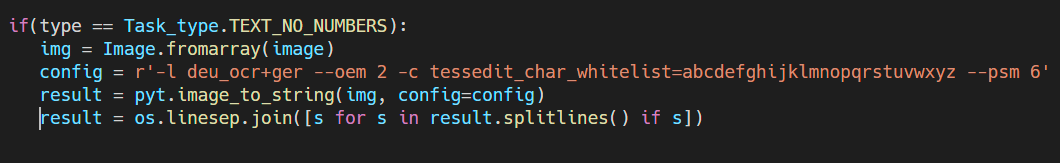
\includegraphics[width=0.8\textwidth]{predict_with_tess}
	\caption[Prediction with tesseract]{predictions of the images using tesseract} \label{Abb:predict_with_tesseract}
\end{figure}